\appendix
\chapter{Topologia de la subestacion gemela}

\section{Diagrama unifilar}

La figura~\ref{fig:unifilar} muestra el diagrama unifilar de la
subestacion modelada en este trabajo. Es representativa de una SE
de distribucion urbana 110/23~kV.

\begin{figure}[ht]
\centering
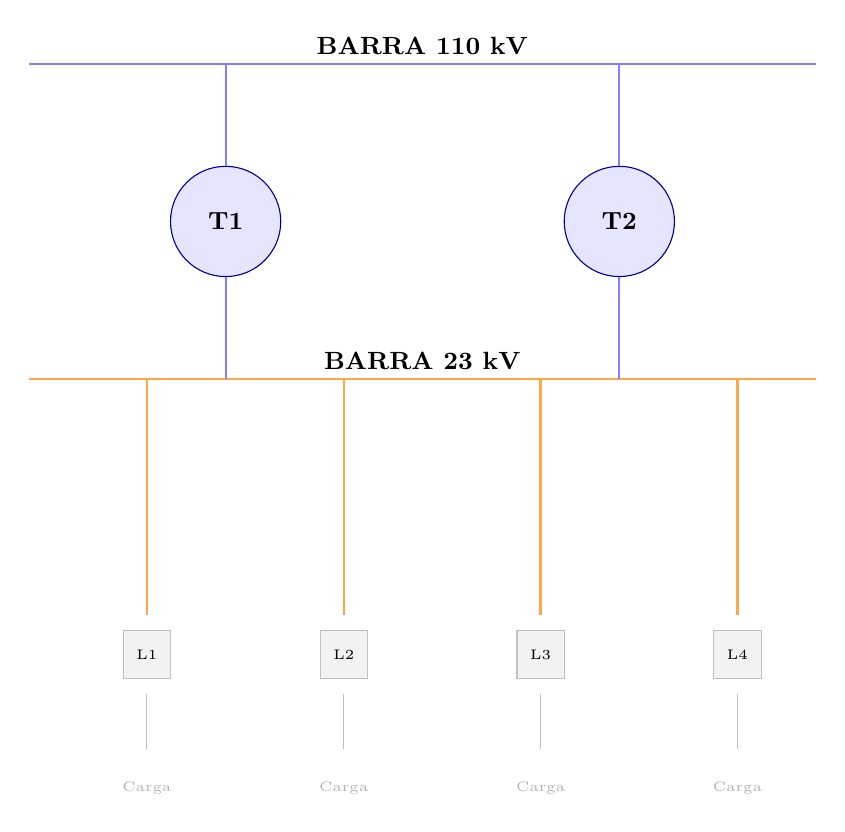
\begin{tikzpicture}[
  every node/.style={font=\small},
  trafo/.style={circle, draw=blue!60!black, fill=blue!10, minimum size=14mm, font=\small\bfseries},
  line/.style={thick, blue!50},
  bt/.style={thick, orange!70},
  load/.style={rectangle, draw=gray!50, fill=gray!10, minimum size=6mm, font=\tiny}
]
% Barras
\draw[line] (0,0) -- (10,0);
\node[above] at (5,0) {\textbf{BARRA 110 kV}};

% Trafos
\node[trafo] (T1) at (2.5,-2) {T1};
\node[trafo] (T2) at (7.5,-2) {T2};
\draw[line] (2.5,0) -- (T1);
\draw[line] (7.5,0) -- (T2);

% Barra BT
\draw[bt] (0,-4) -- (10,-4);
\node[above] at (5,-4) {\textbf{BARRA 23 kV}};

\draw[line] (T1) -- (2.5,-4);
\draw[line] (T2) -- (7.5,-4);

% Alimentadores
\foreach \x/\name in {1.5/L1, 4/L2, 6.5/L3, 9/L4} {
  \draw[bt] (\x,-4) -- (\x,-7);
  \node[load] at (\x,-7.5) {\name};
  \draw[gray!50] (\x,-8) -- (\x,-8.7);
  \node[gray!60, font=\tiny] at (\x,-9.2) {Carga};
}
\end{tikzpicture}
\caption{Diagrama unifilar de la SE 110/23~kV con dos transformadores
y cuatro alimentadores.}
\label{fig:unifilar}
\end{figure}

\section{Parametros completos}

\begin{table}[ht]
\centering
\small
\caption{Parametros electricos completos de la SE gemela.}
\label{tab:param-completa}
\begin{tabular}{ll}
\toprule
\textbf{Parametro} & \textbf{Valor} \\
\midrule
Tension nominal AT  & 110 kV \\
Tension nominal BT  & 23 kV \\
Numero de trafos     & 2 (paralelo) \\
Potencia nominal por trafo & 30 MVA \\
Reactancia de cortocircuito & 0.12 pu \\
Resistencia de cortocircuito & 0.005 pu \\
Perdidas en hierro (Pfe) & 35 kW \\
Perdidas en cobre nominales (Pcu,nom) & 180 kW \\
Constante termica del devanado & 90 min \\
Numero de lineas BT & 4 \\
Longitud L1 & 8 km \\
Longitud L2 & 12 km \\
Longitud L3 & 10 km \\
Longitud L4 & 14 km \\
R linea (pu) L1..L4 & 0.04, 0.06, 0.05, 0.07 \\
X linea (pu) L1..L4 & 0.08, 0.10, 0.09, 0.11 \\
Tension minima de operacion & 0.93 pu \\
Tension maxima de operacion & 1.07 pu \\
Frecuencia minima & 49.5 Hz \\
Frecuencia maxima & 50.5 Hz \\
Temperatura maxima devanado & 95 \si{\degree}C} \\
Corriente maxima por linea & 800 A \\
\bottomrule
\end{tabular}
\end{table}

\section{Cadencia de las mediciones}

\begin{table}[ht]
\centering
\small
\caption{Cadencia de las senales SCADA y PMU.}
\label{tab:cadencia}
\begin{tabular}{lccc}
\toprule
\textbf{Senal} & \textbf{Cadencia} & \textbf{Origen} & \textbf{Uso} \\
\midrule
Tension AT / BT    & 1 Hz   & SCADA & Observada + gemelo \\
Corriente por linea & 1 Hz   & SCADA & Observada + gemelo \\
Potencia activa / reactiva & 1 Hz & SCADA & Observada + gemelo \\
Temperatura devanado T1, T2 & 0.1 Hz & RTU & Termica del gemelo \\
Frecuencia f & 20 Hz & PMU & ROCOF + gemelo \\
ROCOF & 20 Hz & PMU & Conformal \\
THD V, THD I & 1 Hz & SCADA & Calidad de potencia \\
\bottomrule
\end{tabular}
\end{table}

\section{Modelo de estado estacionario}

El flujo de potencia simplificado en regimen permanente asume
sistema equilibrado. Las corrientes por linea se calculan como:

\[
I_k = \frac{S_k}{\sqrt{3} \cdot V_{BT} \cdot V_{k,p}}
\]

donde $S_k$ es la potencia aparente de la linea $k$ y $V_{k,p}$ es
la tension en bornes del alimentador aguas abajo. La caida de
tension en la linea es:

\[
\Delta V_k = \frac{R_{linea,k} \cdot P_k + X_{linea,k} \cdot Q_k}{S_{nom}}
\]

Las perdidas en los transformadores son:

\[
P_{Cu,traf} = 2 \cdot P_{Cu,nom} \cdot \left(\frac{S_{tot}}{2 \cdot S_{nom}}\right)^2
\]
\[
P_{Fe,traf} = 2 \cdot P_{Fe}
\]

La potencia activa solicitada al lado AT es:

\[
P_{AT} = \sum_{k=1}^{4} P_k + P_{Cu,traf} + P_{Fe,traf}
\]

\section{Modelo termico de los devanados}

\[
C_{term} \cdot \frac{dT_{dev}}{dt} = P_{Cu}(t) - h \cdot (T_{dev} - T_{amb})
\]

con:
\begin{itemize}[leftmargin=*,itemsep=2pt]
  \item $P_{Cu}(t) = P_{Cu,nom} \cdot (S_{pu})^2$
  \item $S_{pu} = S_{tot} / (2 \cdot S_{nom})$
  \item $h = 350$ W/\si{\degree}C} (coeficiente de conveccion)
  \item $T_{amb} = 25$ \si{\degree}C} (temperatura ambiente nominal)
  \item $C_{term} = h \cdot \tau_{term} = 350 \cdot 5400 = 1.89$~MW$\cdot$s/\si{\degree}C}
\end{itemize}

Esta dinamica captura el calentamiento lento del devanado bajo
sobrecarga y su enfriamiento tras un evento.